% !TEX root = ../../main.tex
\section{Implementation}\label{sec:vigra_graph_lib_impl}

The most important concept for graph based image processing
is the \emph{region adjacency graph} (RAG) (see \cref{fig:make_rag}).

A RAG is extracted from a labeled \emph{base graph}.
In the first step of graph based image processing, the base 
graph is usually a grid graph, and the labeling is a label image
as in \cref{fig:make_rag} .
To encode a RAG we need a undirected graph, 
and a mapping from the base graphs edges and nodes to the RAG 
needs to be stored.

The implementation of grid graphs is explained in \cref{sec:graphs_grid_graph}, 
a basic undirected graphs implementation will be discussed in \cref{sec:graphs_adjacency_list_graph}.
The implementation details of the \emph{region adjacency graph} concept will 
be given in  \cref{sec:graphs_rag}.

For hierarchical clustering we provide a specialized graph, named \emph{merge graph}.


To implemented structured clustering algorithms (see \cref{sec:rw_hc} we
need a graph which supports the contraction of edges.
Also a mechanism to merge node and edge features is needed.
Within \cref{sec:graphs_merge_graph} we propose  a very flexible
and concept for hierarchical clustering based on a specialized graph,
called \emph{merge graph}.


A generic set of algorithms which work on any graph
implemented within the VIGRA graph api is presented 
in \cref{sec:graph_graph_algorithms}.

While the core implementation of any algorithm is in C++
VIGRA provides python binding to make almost
any algorithm available in Python.
To provide a generic Python interface for any proposed
graph, we need to introduce a few concepts 
to make the python wrapped graph API very \emph{Pythonic}


\subsection{Graphs}


\subsubsection{Grid Graph} \label{sec:graphs_grid_graph}

\missingfigure{show grid graph here}

    \lstinline{vigra::GridGraph<DIM,DIRECTED_TAG>}

\subsubsection{Adjacency List Graph} \label{sec:graphs_adjacency_list_graph}


    \begin{minipage}{\textwidth}\vspace{-0.75cm}\begin{lstlisting}[language=c++]
    typedef AdjacencyListGraph Graph;

    // construct graph
    Graph g;

    // add nodes (id will be asigned automatically)
    Graph::Node n0 = g.addNode() 

    // add node with an explicit id
    Graph::Node n3 = g.addNode(3)

    // add edges from existing nodes
    Graph::Edge e0 = g.addEdge(n0,n1)

    // add edges and nodes simultaneous 
    Graph::Edge e1 = g.addEdge(2,3)

    // no parallel edges 
    Graph::Edge e2 = g.addEdge(2,3)
    assert(e1==e2)  
    \end{lstlisting}\end{minipage}\vspace{0.5cm}



\subsubsection{Region Adjacency Graph} \label{sec:graphs_rag}








To map edges and nodes from the base graph


\subsubsection{Merge Graph} \label{sec:graphs_merge_graph}
To implemented structured clustering algorithms (see \cref{???}) we
need a graph which supports the contraction of edges.
Also a mechanism to merge node and edge features is needed.
Experiments suggest that the edge contraction is more expensive
than feature merging an can even be a bottleneck for huge 3D data 
(see \cref{???} ).
Therefore it is crucial to implemented the MergeGraph (MG) very carefully.
\begin{figure}
    \centering
    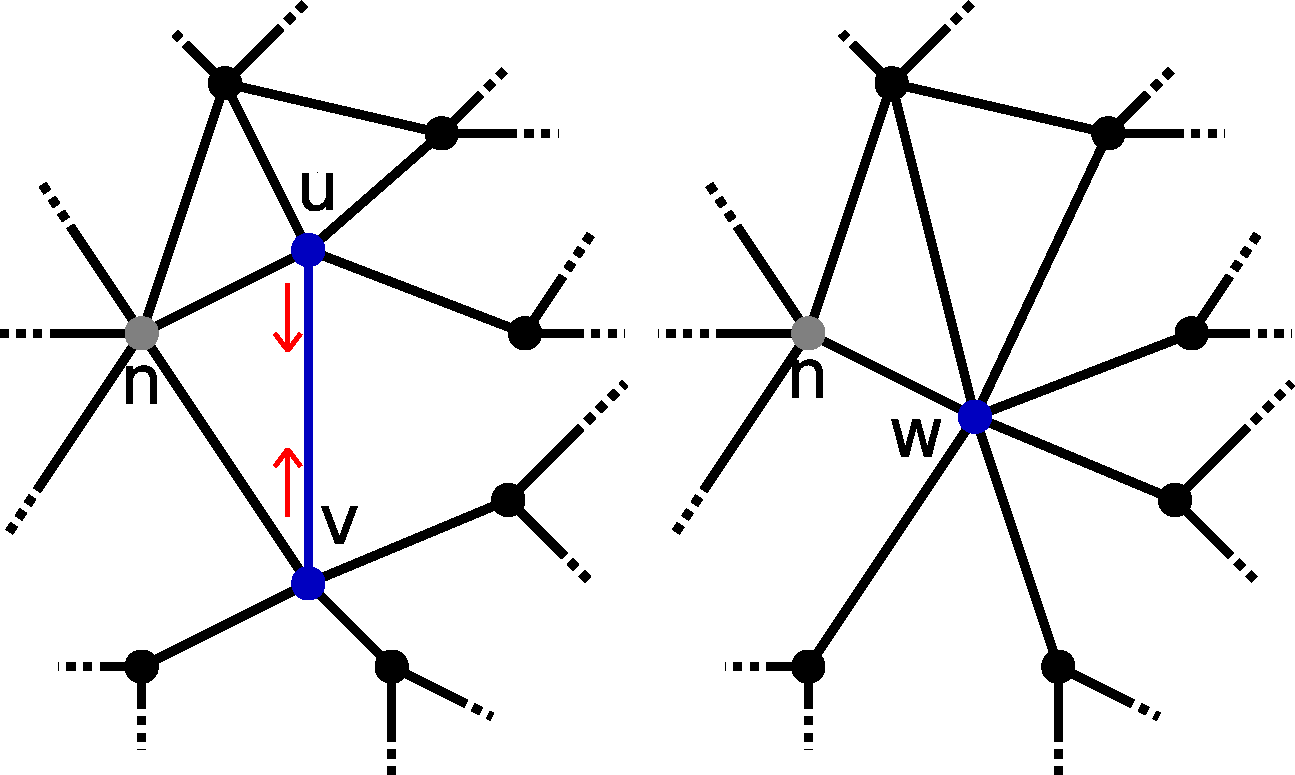
\includegraphics[width=0.35\textwidth]{fig/contraction.pdf}

    \addtocontents{lof}{%
        \vspace{1cm}
        \protect\centerline{%
            \protect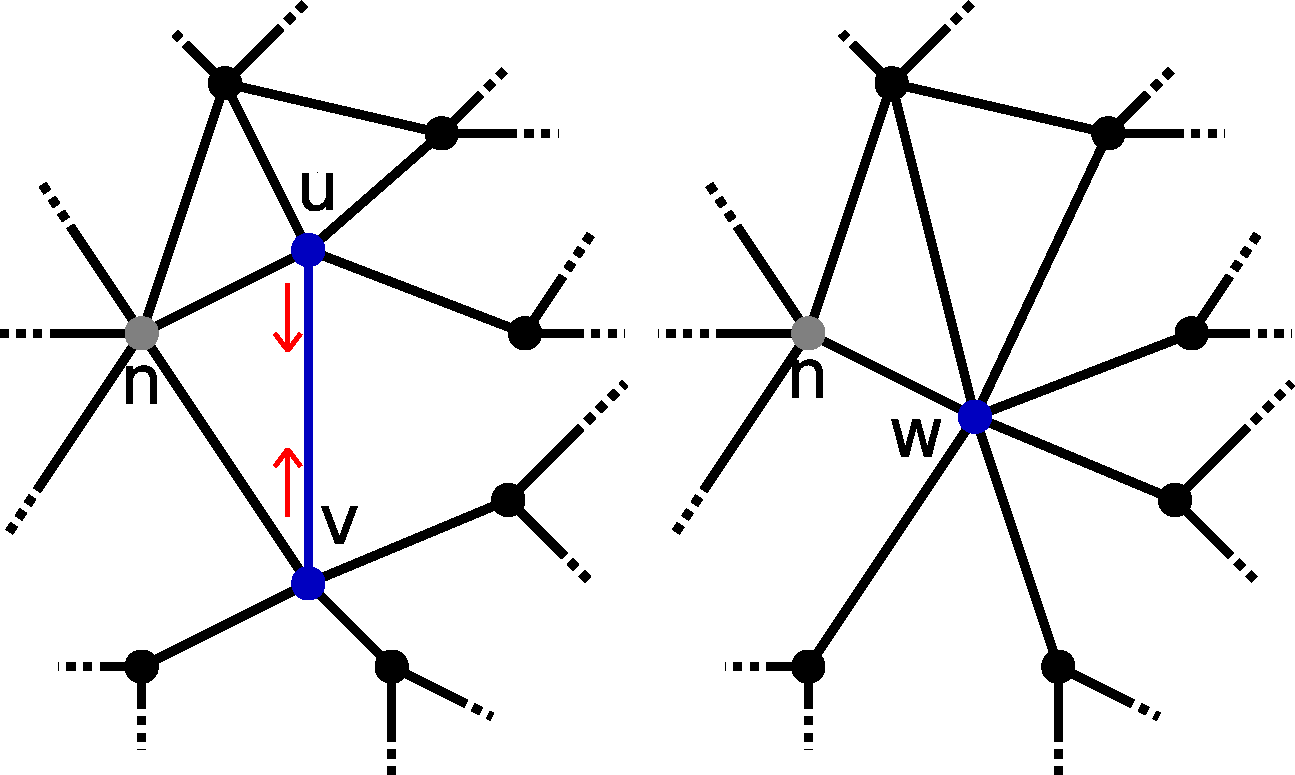
\includegraphics[width=\lofthumbsize,height=\lofthumbsize,keepaspectratio=true]{fig/contraction.pdf} 
        } 
    }%

    %\addtocontents{lof}{%
    %    $\vcenter to \lofthumbsize{\vss%
    %        \hbox to \lofthumbsize {
    %            \hss \protect 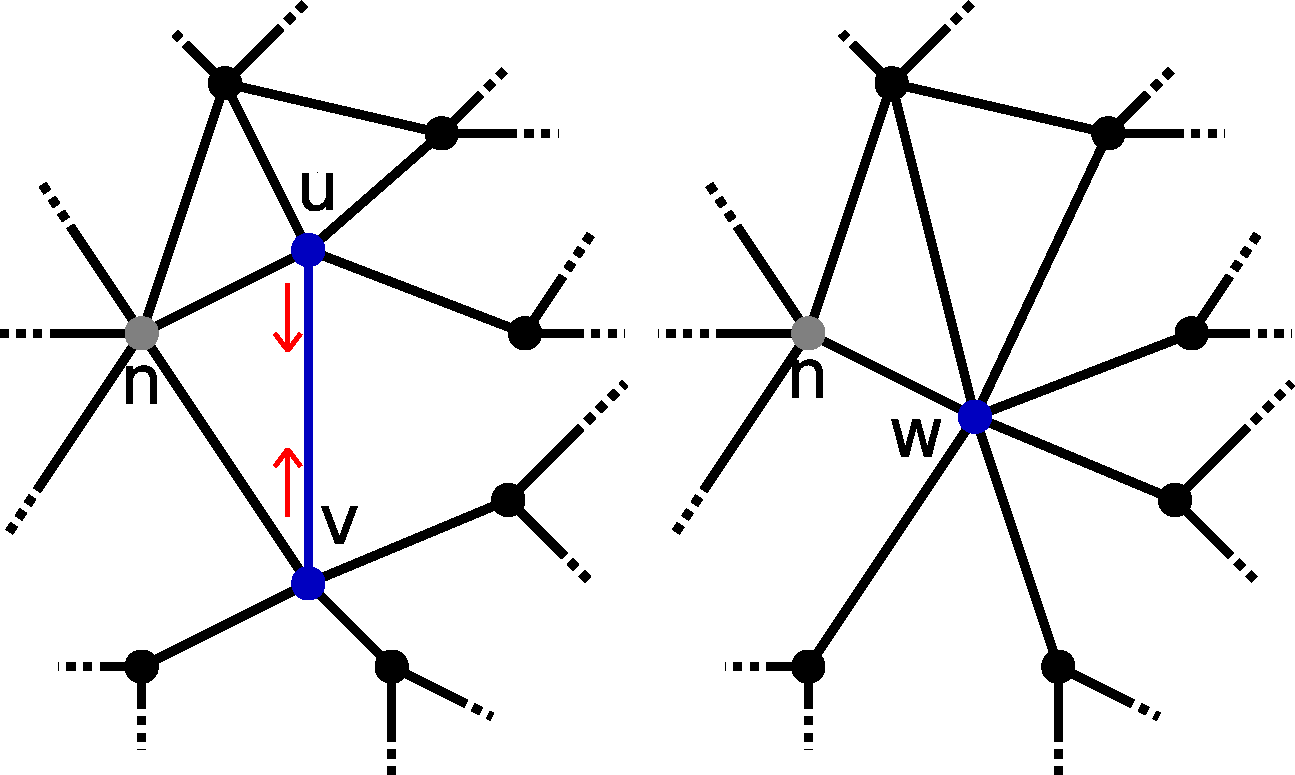
\includegraphics[width=.075\linewidth]{fig/contraction.pdf} \hss
    %        }
    %    \vss}$%
    %    \quad
    %    \ignorespaces
    %}%
    \caption[Schematic edge contraction]{ Schematic edge contraction: Node $u$ and $v$ is merged into node $w$.
        Note the gray node $n$ which is connected to $u$ and $v$.
        After the contraction, edges $\{ n,u\}$ and $\{ n,v\}$ are also merged into 
        a single edge $\{ n, w\}$ 
    }
    \label{fig:figlabel}
\end{figure}


   

\begin{center}
    \begin{tikzpicture}
        \umlclass[template=Graph]{MergeGraphAdpator}
        {
            \\// union find data structures                     \\
            - edgeUfd               : IterablePartiton          \\
            - nodeUfd               : IterablePartiton          \\ 
            - nodesAdjacency        : AdjacencySetVector        \\

            \\// callbacks                                      \\
            - mergeNodeCallBacks    : MergeNodeCallBackVector   \\
            - mergeEdgeCallBack     : MergeEdgeCallBackVector   \\
            - eraseEdgeCallBack     : EraseEdgeCallBackVector   \\
        }
        {
            \\// LEMON API for undirected graphs                \\
                $\ldots$                                        \\
            \\// register callbacks                             \\ 
            + registerMergeNodeCallBack(f : MergeNodeCallBack)  \\
            + registerMergeEdgeCallBack(f : MergeEdgeCallBack)  \\
            + registerEraseEdgeCallBack(f : EraseEdgeCallBack)  \\

            \\// modify graph                                   \\
            + contractEdge(edge : Edge)     : Node              \\

            \\// find representatives                           \\
            + reprNode(node : Node)         : Node              \\
            + reprEdge(edge : Edge)         : Edge              \\ 

            \\// get base graph                                 \\
            + graph()                       : Graph             \\
        } 
    \end{tikzpicture}
\end{center}

\begin{center}
    \begin{tikzpicture}
        \umlclass[template=MergeGraph]{ClusterOperatorInterface}
        {

        }
        {
            \\// contract next edge and get weight              \\
            + contractionEdge(edge : Edge)         : Edge       \\ 
            + contractionWeight(edge : Edge)       : Edge       \\
            \\// get base graph                                 \\
            + mergeGraph()                  : MergeGraph        \\
        } 
    \end{tikzpicture}
\end{center}

\begin{center}
    \begin{tikzpicture}
        \umlclass[template=ClusterOperator]{HierarchicalClustering}
        {

        }
        {
            + cluster()                     : void        \\
            + reprLabels(nodeMap : NodeMap) : void        \\      
        } 
    \end{tikzpicture}
\end{center}


   We propose and implemented the following design:
   \begin{compactitem}
       \item  A base graph is attached to a merge graph  and  a merge graph will
            always ``view'' to
       \item  Union find data structure for nodes
       \item  Union find data structure for edges
   \end{compactitem}



   \lstinline{vigra::MergeGraphAdaptor<DIM,DIRECTED_TAG>}


\subsection{Graph Algorithms} \label{sec:graph_graph_algorithms}

    \subsubsection{Multicut}

    \subsubsection{Hierarchical Clustering}

    \subsubsection{Mst Algorithms}

    \subsubsection{Watershed Algorithms}

    \subsubsection{Smoothing Algorithms}

